\subsection{Functional failure study}
\label{sec:failure-case-study}

%TODO: Speak about impact (or no) of positive stress. Say that only neg stress causes a restart
% What is the failure
The failure is observed on the V\textsubscript{2p5} output pin (Fig. \ref{fig:meas-reset-v2p5}).
It appears when injecting this stress amplitude width etc

The battery is replaced by the injection + DC system

capacitively coupled TLP + isolated DC supply

% What is the root cause -> reset of regulator, soft-start
It seems that the negative stress is causing an unwanted \gls{soft-start} sequence in the regulator.
A soft-start normally happens only during system power-up, when the main external supply is switched on.
During a soft-start, the supply voltage slowly rises from 0V to its nominal value.
It avoids overshoots that could damage sensitive blocks.
By design, soft-starts require a large amount of time to complete, in the range of tens to hundreds microseconds.
As a consequence, the function is not available, or at least not considered valid, until the soft-start is finished.

% How is the test conducted
To generate the negative stress, a \gls{tlp} generator is employed.
The simulations use the \gls{tlp} model described previously in section \ref{sec:tlp-modeling}).
%TODO: reference for DPI
The injection is performed with a \gls{bias-tee}, similarly to the DPI standard.
The stress generator and DC supply are isolated from one another with a capacitor-inductor network (Fig. \ref{fig:injection-setup-dpi}).

\begin{figure}[!h]
  \centering
  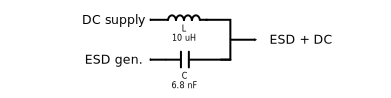
\includegraphics{src/3/figures/injection_setup_dpi.pdf}
  \caption{Injection setup to superimpose a stress on a DC voltage}
  \label{fig:injection-setup-dpi}
\end{figure}

Failure It affects the behavior of the entire system, because this net powers many other functions in the system.
The failure is induced by injecting a large negative-voltage stress on the input V\textsubscript{batt}, when the product is in operation.
The discharge is superimposed on a DC voltage value.
This input is a realistic entry point for \gls{esd} in the integrated circuit, because it is exposed at the system level and connected to the battery by a cable.
The disturbance on the output V\textsubscript{2p5} is much longer (30 \textmu{}s) than on the input V\textsubscript{batt} (100 ns).

\begin{figure}[!h]
  \centering
  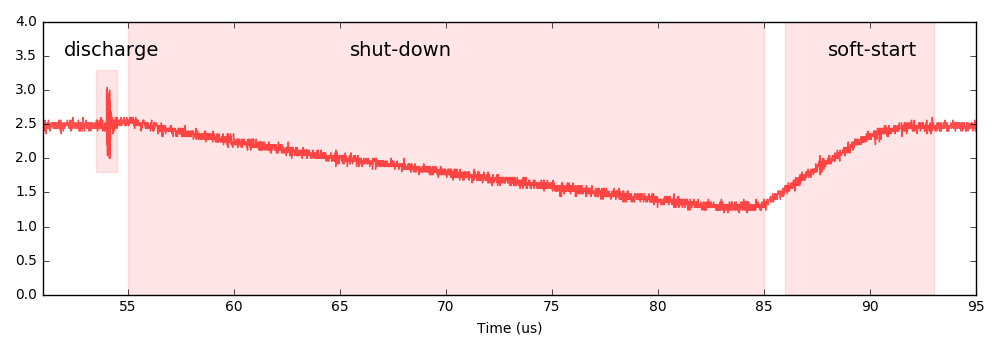
\includegraphics[width=0.9\textwidth]{src/3/figures/v2p5_measure.png}
  \caption{Measurement of V\textsubscript{2p5} after a -450V 100ns negative stress}
  \label{fig:meas-reset-v2p5}
\end{figure}


% Compare sim and meas for Vbatt
The simulation of V\textsubscript{batt} is compared with a measurement in Fig. \ref{fig:wvf-vbatt}.
During the discharge, V\textsubscript{batt} has a larger amplitude in simulation, and reaches a more negative voltage.
The positive overshoot after the pulse is correctly reproduced, although it dampens slower in the simulation.
Overall, the accuracy is rather satisfying.

% Compare sim and meas for V2p5
Fig. \ref{fig:wvf-v2p5} provides the same comparison for V\textsubscript{2p5}.
The reset is clearly visible on both curves.
The restart happens almost at the same time in both waveforms, about 32\textmu{}s after the stress was injected.
Right after the \gls{esd} injection, the disturbance amplitude is a bit larger in simulation.
But overall, the accuracy is satisfying.
Both comparisons tend to indicate that simulations can be trusted to reproduce the failure in this study case.

\begin{figure}[!h]
  \centering
  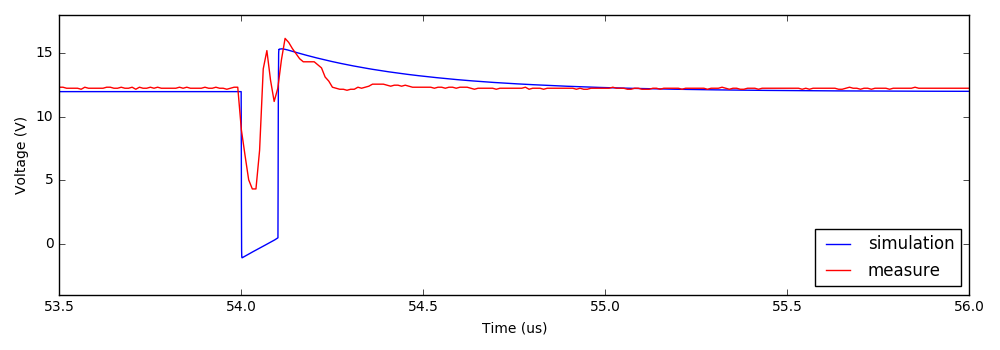
\includegraphics[width=0.95\textwidth]{src/3/figures/vbatt.png}
  \caption{Measurement and simulation for V\textsubscript{batt}}
  \label{fig:wvf-vbatt}
\end{figure}

\begin{figure}[!h]
  \centering
  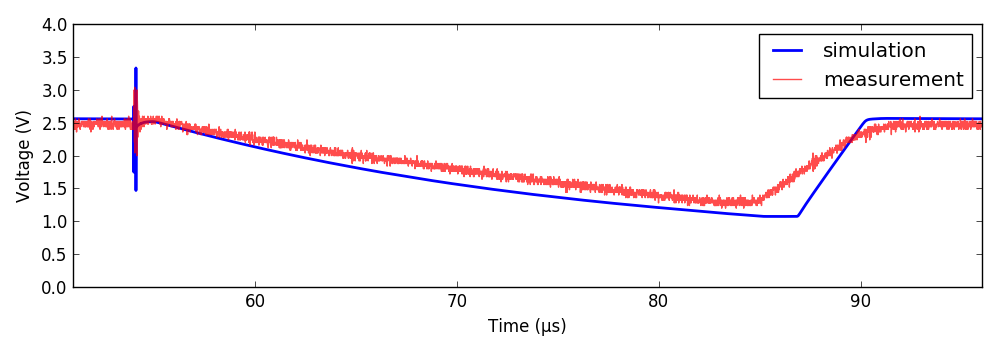
\includegraphics[width=0.9\textwidth]{src/3/figures/v2p5.png}
  \caption{Measurement and simulation of the functional failure on V\textsubscript{2p5}}
  \label{fig:wvf-v2p5}
\end{figure}

% Now use the simulation for analysis
Simulations are employed to observe the intermediate nets, that are hard to access and measure physically.
In the first simulation, a rectangular pulse of -100V amplitude and 100 ns width in injected once again on V\textsubscript{batt}.
The waveform for output V\textsubscript{clamp9} of the pre-regulator is given in Fig. \ref{fig:wvf-vclamp9}.
At 54 \textmugreek{}s,  V\textsubscript{clamp9} is disturbed by the negative stress, in two phases.
The first phase is 100 ns wide, and corresponds to the direct exposure to the stress.
During this phase, V\textsubscript{clamp9} reaches as low as 0V for a brief amount of time.
Afterwards, there is a second phase, that lasts approximately 650 ns.
The reason for this second undervoltage is not clearly known, but it looks similar to the positive overshoot on the  V\textsubscript{batt} curve (Fig. \ref{fig:wvf-vbatt}).
Overall, V\textsubscript{clamp9} is disturbed for 750 ns.

\begin{figure}[!h]
  \centering
  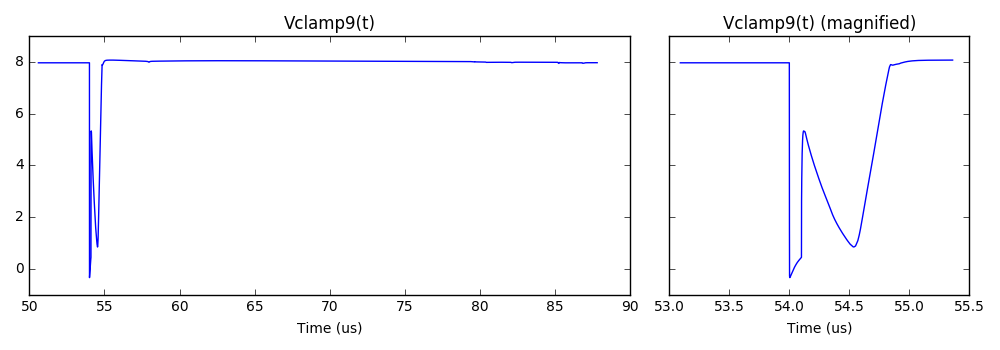
\includegraphics[width=0.95\textwidth]{src/3/figures/vclamp9.png}
  \caption{Simulated waveform of the V\textsubscript{clamp9} internal net}
  \label{fig:wvf-vclamp9}
\end{figure}

% Next net, bandgap input
V\textsubscript{clamp9} is the output of the pre-regulator, and is a power-supply input for the bandgap reference.
The bandgap is expected to be disturbed because of the variation on V\textsubscript{clamp9}.
The observation of the 1.0V bandgap reference V\textsubscript{ref1p0} confirms it (Fig. \ref{fig:wvf-v1p0}).
The reference drops down to 0.25V, and is disturbed for about 3 \textmugreek{}s.

\begin{figure}[!h]
  \centering
  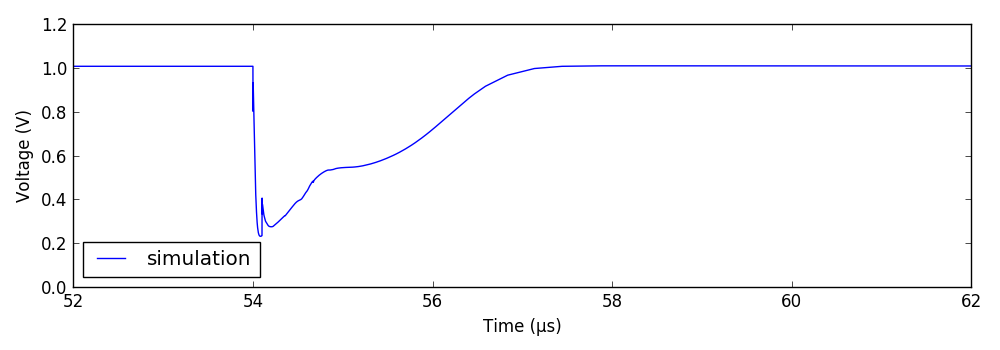
\includegraphics[width=0.9\textwidth]{src/3/figures/v1p0.png}
  \caption{Simulated waveform of the V\textsubscript{ref1p0} internal net}
  \label{fig:wvf-v1p0}
\end{figure}

% Final net
Finally, V\textsubscript{ref1p0} is used by the regulator to generate the 2.5 V external supply output V\textsubscript{2p5}.
Previously,  Fig. \ref{fig:wvf-v2p5} showed that V\textsubscript{2p5} drops below 1.5V, and is disturbed for more than 30 \textmugreek{}s.

% Preliminary conclusion with scale factor
There is a clear trend regarding the duration of the failure.
In the first block (pre-regulator), the disturbance width increased from 100 ns to 750 ns.
In the second block (bandgap), it increased from 750 ns to 3 \textmugreek{}s.
In the third block (regulator), it reached 30 \textmugreek{}s.
Each time, there is an aggravation of the failure.

% Talk about failure in cascade
It appears there is a failure in cascade of the regulation function.
When the disturbance propagates through a block, it is somehow amplified and becomes more severe.
Ultimately, a function that takes a lot of time to recover (soft-start) is hit, causing a full system restart.

% Transition
The next part of this research work is focused on developping measurement methods to acquire data on silicon, to confirm the simulations.
A testchip is designed to test new measurement and observation methods in section \ref{sec:test-vehicle-desc}.
Modeling methods are explored in section \ref{sec:bottom-up-modeling} as a way to understand and predict these functional issues.
